% Architecture overview for the README.
% Regenerate the committed SVG after editing:
%   pdflatex architecture.tex && pdftocairo -svg architecture.pdf architecture.svg
\documentclass[tikz,border=10pt]{standalone}
\usepackage[scaled]{helvet}
\renewcommand{\familydefault}{\sfdefault}
\usetikzlibrary{arrows.meta,backgrounds,calc,fit,positioning}
\pgfdeclarelayer{zones}
\pgfdeclarelayer{innerzones}
\pgfsetlayers{background,zones,innerzones,main}

\definecolor{ink}{HTML}{263238}
\definecolor{boxline}{HTML}{90A4AE}
\definecolor{traffic}{HTML}{37474F}
\definecolor{dial}{HTML}{546E7A}
\definecolor{dep}{HTML}{8D6E63}
\definecolor{netLine}{HTML}{5E35B1}
\definecolor{netFill}{HTML}{EDE7F6}
\definecolor{cfLine}{HTML}{E65100}
\definecolor{cfFill}{HTML}{FFF3E0}
\definecolor{vpsLine}{HTML}{1565C0}
\definecolor{vpsFill}{HTML}{E3F2FD}
\definecolor{homeLine}{HTML}{2E7D32}
\definecolor{homeFill}{HTML}{EEF7EF}
\definecolor{piLine}{HTML}{F9A825}
\definecolor{piFill}{HTML}{FFFDE7}
\definecolor{k8sLine}{HTML}{0277BD}
\definecolor{k8sFill}{HTML}{E1F5FE}

\begin{document}
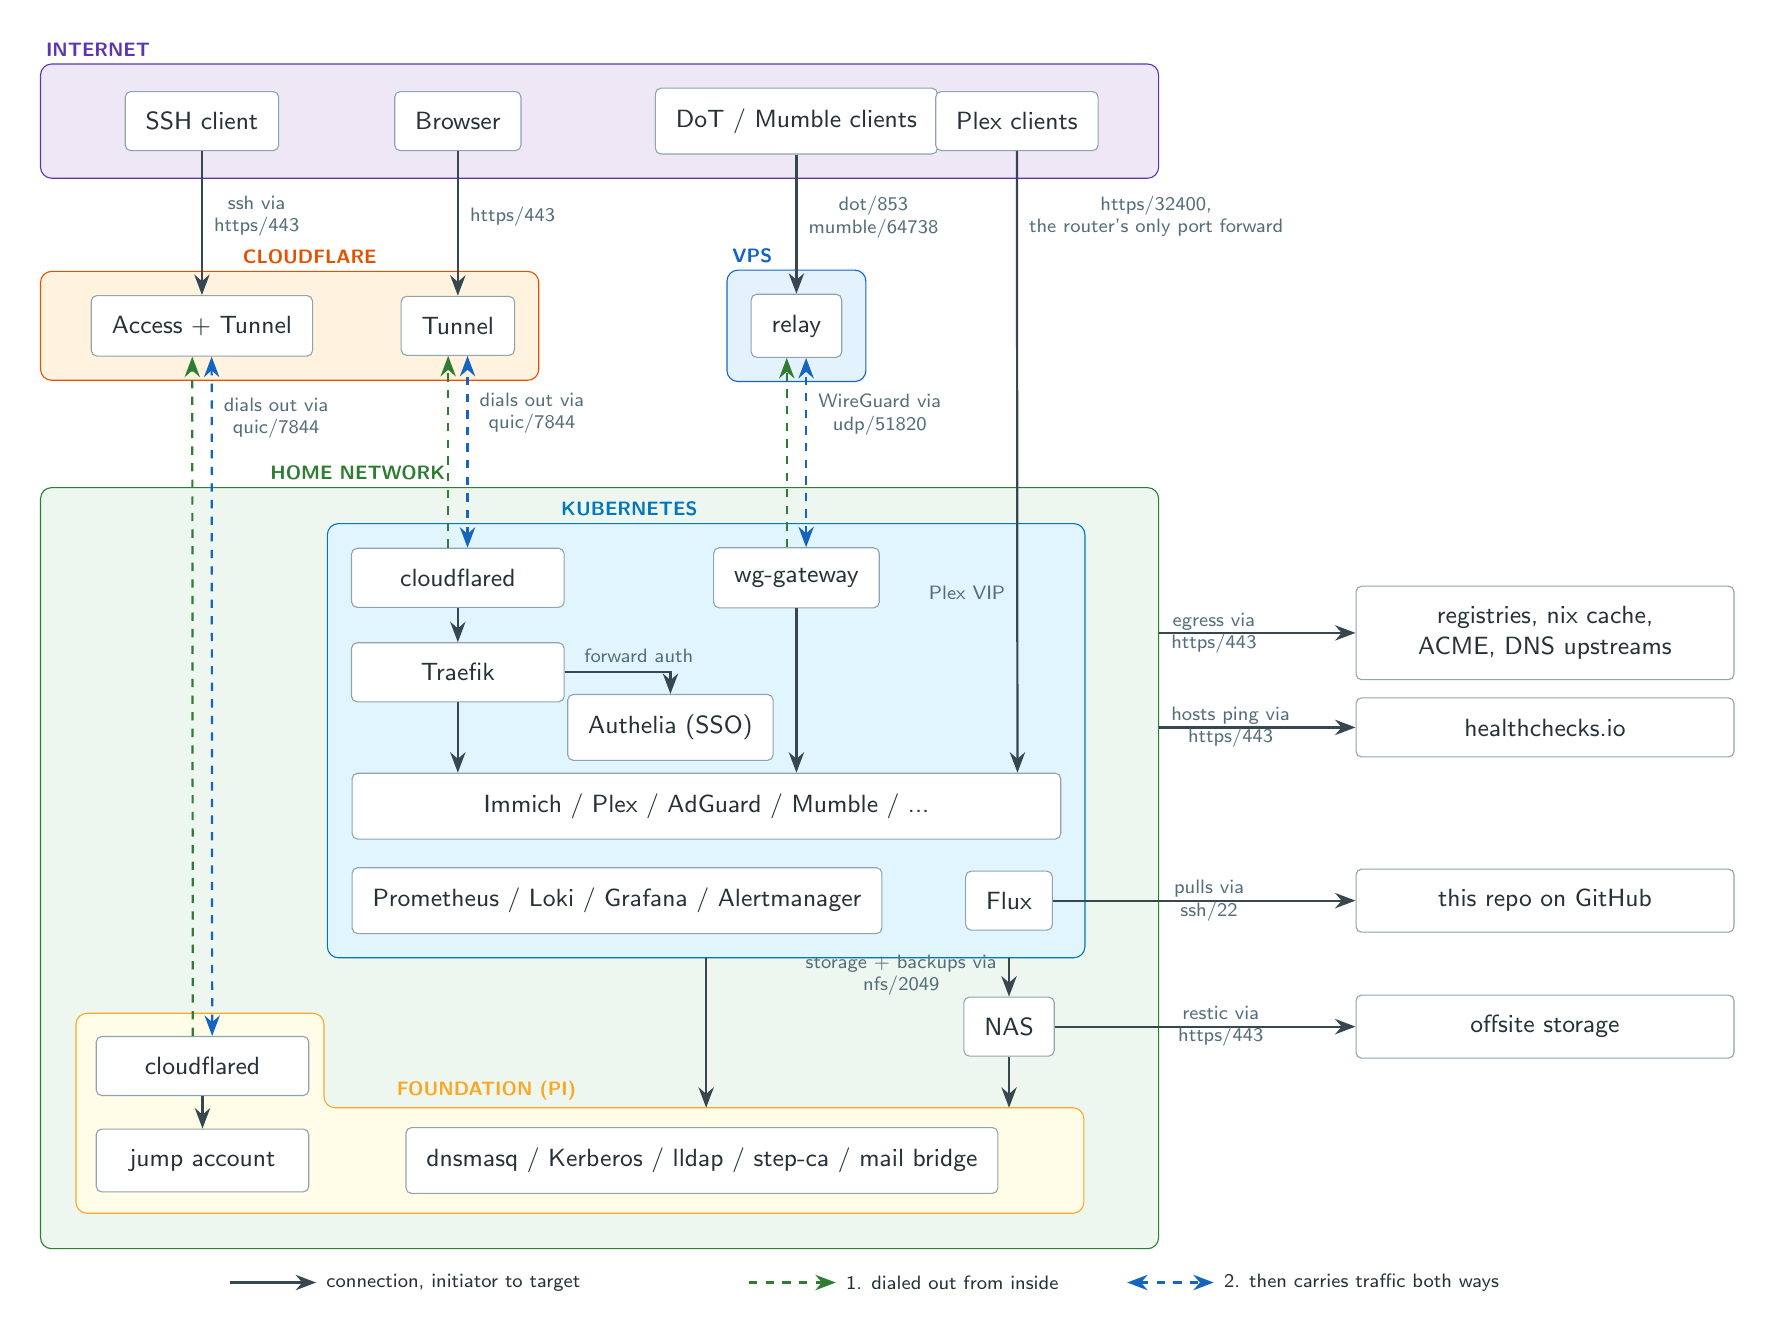
\begin{tikzpicture}[
    background rectangle/.style={fill=white, rounded corners=10pt},
    show background rectangle,
    box/.style={draw=boxline, fill=white, text=ink, rounded corners=2pt,
                minimum height=7.5mm, inner sep=2.6mm, font=\small},
    zone/.style={rounded corners=4pt, inner sep=3mm},
    ztab/.style={font=\scriptsize\bfseries, fill=none, inner xsep=0.2mm,
                 inner ysep=1pt, anchor=south west},
    t/.style={-{Stealth[length=2.6mm]}, draw=traffic, thick},
    d1/.style={-{Stealth[length=2.6mm]}, draw=homeLine, thick, dashed},
    d2/.style={{Stealth[length=2.6mm]}-{Stealth[length=2.6mm]}, draw=vpsLine,
               thick, dashed},
    el/.style={font=\scriptsize, text=dial, fill=none, inner sep=1pt, align=center},
  ]

  % ---- internet row -------------------------------------------------------
  \node[box] (sshc)  at (-0.35,0)  {SSH client};
  \node[box] (brow)  at (2.9,0)   {Browser};
  \node[box] (dotc)  at (7.2,0)   {DoT / Mumble clients};
  \node[box] (plexc) at (10.0,0)  {Plex clients};

  % ---- cloud row ----------------------------------------------------------
  \node[box] (access) at (-0.35,-2.6) {Access + Tunnel};
  \node[box] (tunnel) at (2.9,-2.6) {Tunnel};
  \node[box] (relay)  at (7.2,-2.6) {relay};

  % ---- home: kubernetes ---------------------------------------------------
  \node[box, minimum width=27mm] (cfd) at (2.9,-5.8) {cloudflared};
  \node[box] (wgw)     at (7.2,-5.8)  {wg-gateway};
  \node[box, minimum width=27mm] (traefik) at (2.9,-7.0) {Traefik};
  \node[box] (auth)    at (5.6,-7.7)  {Authelia (SSO)};
  \node[box, anchor=west, minimum width=90mm] (apps) at (1.55,-8.7)
      {Immich / Plex / AdGuard / Mumble / ...};
  \node[box] (flux)    at (9.9,-9.9) {Flux};
  \node[box, anchor=west] (mon) at (1.55,-9.9)
      {Prometheus / Loki / Grafana / Alertmanager};

  % ---- home: rest ---------------------------------------------------------
  \node[box, anchor=west, minimum width=27mm] (cfdp) at (-1.7,-12.0) {cloudflared};
  \node[box, anchor=west, minimum width=27mm] (jump) at (-1.7,-13.2) {jump account};
  \node[box] (infra) at (6.0,-13.2)
      {dnsmasq / Kerberos / lldap / step-ca / mail bridge};
  \node[box] (nas)    at (9.9,-11.5) {NAS};

  % ---- external -----------------------------------------------------------
  \node[box, align=center, anchor=west, minimum width=48mm] (upst) at (14.3,-6.5)
      {registries, nix cache,\\ACME, DNS upstreams};
  \node[box, anchor=west, minimum width=48mm] (repo) at (14.3,-9.9) {this repo on GitHub};
  \node[box, anchor=west, minimum width=48mm] (hc) at (14.3,-7.7) {healthchecks.io};
  \node[box, anchor=west, minimum width=48mm] (offsite) at (14.3,-11.5) {offsite storage};

  % ---- zones --------------------------------------------------------------
  \coordinate (netL) at (-2.1,0);
  \coordinate (netR) at (11.5,0);
  \coordinate (cfL) at (-2.1,-2.6);
  \coordinate (piTL) at (-1.95,-11.33);
  \coordinate (piBR) at (10.85,-13.87);
  \coordinate (homeR) at (11.35,-8.0);
  \begin{pgfonlayer}{innerzones}
    \node[zone, draw=netLine, fill=netFill, fit=(sshc)(brow)(dotc)(plexc)(netL)(netR)] (znet) {};
    \node[zone, draw=cfLine, fill=cfFill, fit=(access)(tunnel)(cfL)] (zcf) {};
    \node[zone, draw=vpsLine, fill=vpsFill,
          fit=(relay)] (zvps) {};
    \node[zone, draw=k8sLine, fill=k8sFill,
          fit=(cfd)(wgw)(traefik)(auth)(apps)(flux)(mon)] (zk8s) {};
    \draw[draw=piLine, fill=piFill, rounded corners=4pt]
        (-1.95,-11.33) -- (1.2,-11.33) -- (1.2,-12.53) -- (10.85,-12.53)
        -- (10.85,-13.87) -- (-1.95,-13.87) -- cycle;
  \end{pgfonlayer}
  \begin{pgfonlayer}{zones}
    \node[zone, draw=homeLine, fill=homeFill, inner sep=4.5mm,
          fit=(zk8s)(nas)(homeR)(piTL)(piBR)] (zhome) {};
  \end{pgfonlayer}
  \node[ztab, text=netLine]  at ($(znet.north west)+(0.05,0.05)$) {INTERNET};
  \node[ztab, text=cfLine]   at ($(zcf.north west)+(2.55,0.05)$) {CLOUDFLARE};
  \node[ztab, text=vpsLine]  at ($(zvps.north west)+(0.05,0.05)$) {VPS};
  \node[ztab, text=homeLine] at ($(zhome.north west)+(2.9,0.05)$) {HOME NETWORK};
  \node[ztab, text=k8sLine]  at ($(zk8s.north west)+(2.95,0.05)$) {KUBERNETES};
  \node[ztab, text=piLine]   at (2.1,-12.48) {FOUNDATION (PI)};

  % ---- traffic (solid) ----------------------------------------------------
  \draw[t] (sshc) -- node[el, pos=0.45, anchor=west, xshift=3pt] {ssh via\\https/443} (access);
  \draw[t] (brow) -- node[el, pos=0.45, anchor=west, xshift=3pt] {https/443} (tunnel);
  \draw[t] (dotc) -- node[el, pos=0.45, anchor=west, xshift=3pt] {dot/853\\mumble/64738} (relay);

  \draw[t] (cfd) -- (traefik);
  \draw[t] (traefik) -- (traefik |- apps.north);
  \draw[t] (traefik.east) -| node[el, above=2pt, pos=0.35] {forward auth} (auth.north);
  \draw[t] (wgw) -- (wgw |- apps.north);
  \draw[t] (plexc) -- node[el, pos=0.105, anchor=west, xshift=3pt]
      {https/32400,\\the router's only port forward}
      node[el, pos=0.71, anchor=east, xshift=-3pt] {Plex VIP}
      ([xshift=39.5mm]apps.north);
  \draw[t] (nas.north |- zk8s.south) -- node[el, pos=0.45, anchor=east,
      xshift=-3pt] {storage + backups via\\nfs/2049} (nas.north);

  % ---- dialed out from inside (dashed) ------------------------------------
  \draw[d1] ([xshift=-3.5pt]cfd.north) -- ([xshift=-3.5pt]tunnel.south);
  \draw[d2] ([xshift=3.5pt]cfd.north) -- node[el, pos=0.7, anchor=west,
      xshift=3pt] {dials out via\\quic/7844} ([xshift=3.5pt]tunnel.south);
  \draw[d1] ([xshift=-3.5pt]wgw.north) -- ([xshift=-3.5pt]relay.south);
  \draw[d2] ([xshift=3.5pt]wgw.north) -- node[el, pos=0.7, anchor=west,
      xshift=3pt] {WireGuard via\\udp/51820} ([xshift=3.5pt]relay.south);
  \draw[d1] ([xshift=-3.5pt]cfdp.north) -- ([xshift=-3.5pt]access.south);
  \draw[t] (cfdp) -- (jump);
  \draw[d2] ([xshift=3.5pt]cfdp.north) -- node[el, pos=0.91, anchor=west,
      xshift=3pt] {dials out via\\quic/7844} ([xshift=3.5pt]access.south);
  \draw[t] (flux) -- node[el, pos=0.36, anchor=west, xshift=3pt] {pulls via\\ssh/22} (repo);
  \draw[t] (zhome.east |- upst.west) -- node[el, at start, anchor=west,
      xshift=3pt] {egress via\\https/443} (upst.west);
  \draw[t] (zhome.east |- hc.west) -- node[el, at start, anchor=west, xshift=3pt] {hosts ping via\\https/443} (hc.west);
  \draw[t] (zk8s.south) -- (zk8s.south |- 0,-12.53);
  \draw[t] (nas.south) -- (nas.south |- 0,-12.53);
  \draw[t] (nas) -- node[el, pos=0.37, anchor=west, xshift=3pt] {restic via\\https/443} (offsite);

  % ---- legend -------------------------------------------------------------
  \begin{scope}[shift={(0,-14.75)}]
    \draw[t] (0,0) -- (1.1,0) node[anchor=west, font=\scriptsize, text=ink]
      {connection, initiator to target};
    \draw[d1] (6.6,0) -- (7.7,0) node[anchor=west, font=\scriptsize, text=ink]
      {1. dialed out from inside};
    \draw[d2] (11.4,0) -- (12.5,0) node[anchor=west, font=\scriptsize, text=ink]
      {2. then carries traffic both ways};
  \end{scope}
\end{tikzpicture}
\end{document}
